\chapter{Results}
\label{chapter:Results}

\section{Predicting atomic interactions from 3D structure}
\label{sec:champs}

This section describes my experiments for the Kaggle competition 'Predicting Molecular Properties'~\footnote{\url{https://www.kaggle.com/c/champs-scalar-coupling}} hosted by CHAMPS (CHemistry And Mathematics in Phase Space)
%~\footnote{\url{https://champsproject.com}}.
The dataset and the evaluation are described in Section~\ref{sec:champs-dataset}. Here, it suffices to say that the raw data are 3D structures very much like the ones in the \textit{Alchemy}-dataset (Section~\ref{sec:alchemy-dataset}) but the target variable is an atomic interaction - i.e. an edge property in graph terminology.


\begin{table}[H]
\begin{centering}
	\begin{tabular}{||c | c | c||} 
		\hline
		Experiment & Section & score* \\ [0.5ex] 
		\hline\hline
		\textit{LightGBM} with distance and atom type & \ref{sec:dist-atom-type} & -1.19 \\ 
		\textit{LightGBM} with distance, angle and atom type & \ref{sec:dist-angle-atom-type} & -1.38 \\
		\textit{SchNet} DGL implementation & \ref{sec:schnet} & 0.52  \\
		\textit{SchNet} Chainer-implementation (fine-tuned) & \ref{sec:schnet} & -1.95 \\ [1ex] 
		\hline
	\end{tabular}
	\vspace{0.5cm}
	\caption{Summary of the results of different experiments from the Kaggle competition 'Predicting Molecular Properties'. *The score is based on the MAE and defined in Section~\ref{sec:champs-dataset}.}
	\label{tab:champs-results}
\end{centering}
\end{table}


\subsection{Boosted Tree models with manually engineered features}
\label{sec:champs-boosted-tree}

Simple machine learning models based on manually engineered features, such as various versions of boosted trees can give surprisingly good results with short training time. They do not reach the performance of well tuned MPNNs but easily surpass not yet fully optimized MPNN models. The next two subsection will briefly outline two experiments with manually engineered features used for a Light Gradient Boosted Model (\textit{LightGBM})~\cite{Ke2017}.


\subsubsection{Distance and atom-type features}
\label{sec:dist-atom-type}

The first type of engineered features were calculated in the following way: The center point between the two atoms whose J-coupling constant has to be predicted was calculated (on a straight line). Then, the distances to the ten closest other atoms were calculated and added as features along with the types of the atoms as categorical variables. Finally, the distance between the two J-coupled (interacting) atoms was added to the features as well yielding a total of 21 features. These features were fed into eight different LightGBMs
for the eight different J-coupling types to predict the scalar coupling constant. The models are fitted quickly and give reasonable results without hyper-parameter tuning. The experiment can be easily reproduced by running the publicly available Kaggle-notebook \url{https://www.kaggle.com/rpeer333/super-simple-10-nearest-atoms-features}. The result was decent given the simplicity of the approach but markedly below a well tuned MPNN (see Table~\ref{tab:champs-results}).

Several factors limit the effectiveness of this simple approach.

\paragraph{Lack of geometric information} The features only specify an atoms distance from the center point and not it's position relative to the J-coupled atoms.

\paragraph{Features are not permutation invariant} As atoms in a molecule have no objective order that makes them comparable to other atoms in other molecules (at least in the general case), the feature order is somewhat arbitrary limiting the model's ability to generalize. Granted, some patterns are shared between interactions. E.g. in the case of a J2XX interaction where the J-coupled molecules are two bonds apart, the atom closes to the center point is most likely the atom to which both j-coupled atoms are bound, making the first distance and the first atom-type feature comparable across interactions. But in the general cases, the n\textsuperscript{th} closes atom in an arbitrary interaction is not equivalent to the n\textsuperscript{th} closes atom in another interaction.

\paragraph{Lack of structure within the features} Obviously, the features are not just 21 independent scalars. Instead, the closest atom's distance to the center point is related to this atom's type, etc. However, this relation is not represented when the features are input into the model as 21 independent variables.


\subsubsection{Distance, atom-type and angle features}
\label{sec:dist-angle-atom-type}

Regarding the three limitations in the previous section, this experiment attempted to address the first one. Recall that the distance was calculated from the center point of the straight line between the two J-coupled atoms. In this approach an additional set of features was added to indicate whether a given atom is closer to one or the other of the j-coupled atoms. We define the J-coupled atoms as atom-0 and atom-1. E.g. for the interaction type 1JHC, the hydrogen atom H is always atom-0 and the the carbon atom C is always atom-1. Then, the cosine of the angle between a given atom-x, the center point and atom-1 is added to the features. This feature is automatically scaled between 0 and 1. A feature value close to -1 indicates that atom-x is closer to atom-0 while a value closer to 1 indicates proximity to atom-1. The experiment can be reproduced by running the following Kaggle-notebook:~ \url{https://www.kaggle.com/rpeer333/only-distance-type-and-angle-of-10-nearest-atoms}

Adding this set of features to the ones described in the previous section gave 31 features. While some more (but not all) geometric information is provided in this approach, the other two issues described in the previous section are not addressed by this approach. The results were slightly better than in the above experiment but the difference is not outstanding (see Table~\ref{tab:champs-results}) indicating that the main issues are indeed the two open problems of the features not being permutation invariant and the lack of representation of the relation between features (type of a given atom, it's distance to the center-point and it's cosine).

The same issues would apply to any other manually engineered features. Thus, these results provide good motivation good motivation to explore a MPNN approach shown in the next section.


\subsection{MPNNs for edge property prediction}
\label{sec:schnet}

The \textit{SchNet}~\cite{Schutt2017} model is described using the graph convolution terminology (see Section~\ref{sec:motivation}) but it could equally well be described in the message passing framework proposed by Gilmer et. al.~\cite{Gilmer2017}. The most relevant part of the architecture is the use of what they call \textit{continuous- filter convolutional layers}. In message passing terminology, this refers to the use of the distance as continuous edge feature. In the application of this model to the Kaggle competition at hand, this feature is not thresholded. This means that an edge with distance as edge feature is added between any two atoms in the molecule. In that manner, a complete graph is created where every atom is connected to every other atom in the molecule. It stands to reason that the success of the model might rely on the use of complete graphs rather than on the use of the continuous distance feature. The next section shows a similar example (Section~\ref{sec:neighborhood-expansion}).

In this experiment, a \textit{SchNet} model was implemented using the python library DGL (deep graph library). An implementation in the library \textit{Chainer} for the same competition was used as a template~\footnote{\label{fn:chainer-schnet}\url{https://www.kaggle.com/toshik/schnet-starter-kit}}. Several changes from the template as well as from the paper~\cite{Schutt2017} were implemented and tested but the performance was far off the one from the template as well as the performance of the LightGBM models described above in Section~\ref{sec:champs-boosted-tree} (see Table~\ref{tab:champs-results}). For this reason, no further experiments were conducted with this architecture. The full implementation of the model is available in this notebook: \url{https://www.kaggle.com/rpeer333/pytorch-dgl-schnet-a-graph-convolutional-net}.

Instead, using the template from Footnote~\ref{fn:chainer-schnet} to create eight different models for the eight different J-coupling types was much more effective. Furthermore, adapting the layer-dimension (smaller dimension for less complex interaction types and vice versa) as well as longer training time gave good enough results to achieve a placement in the top 10\% in the competition (see Table~\ref{tab:champs-results})~\footnote{Finishing as proud 198\textsuperscript{th} out of 2749 teams (and awarding a virtual Kaggle-medal).}. The experiments described in this and the previous sections show that achieving competitive results with a truly novel approach would take more experience and more time while simply taking a working solution and adapting it properly to the use-case at hand can give good results with relatively low time investment.


\section{Predicting molecular properties from 3D structure}
\label{sec:alchemy}

During the practical work for this thesis, I participated in the Tencent-Alchemy competition~\footnote{\url{https://alchemy.tencent.com}} using approach described above a baseline architecture. This competition provided a labeled training- and validation-set of as well as an unlabeled test-set of 3D molecular structures described in more detail in Section~\ref{sec:alchemy-dataset}. All remaining experiments in this thesis have been conducted with this dataset.

Despite many experiments (see Table~\ref{tab:alchemy-results}), I achieved the best results simply fine-tuning the model from Chen et. al.\cite{Chen2019} and finished 26th out of 53 participants~\footnote{\url{https://alchemy.tencent.com/\#leaderboard}}. The fact that half the participants did not beat the baseline published in the official competition paper, shows that the approach is indeed quite effective an warrants a closer examination why the peculiar approach of using complete graphs works quite well.

%As discussed in the introduction, a central concept of graph convolution (and regular convolution as well), is to compute a representation of a local neighborhood. In the case of graphs, a local neighborhood is a node and its neighbor nodes while on images, it is a small patch of pixels, such as 3x3 or 5x5.



\begin{table}[H]
\begin{centering}
	\begin{tabular}{||c | c | c||} 
		\hline
		Experiment & Section & MAE \\ [0.5ex] 
		\hline\hline
		base-line (Chen et. al.~\cite{Chen2019})  & \ref{sec:neighborhood-expansion} & 0.0569 \\
		root-node (graph-state) & \ref{sec:root-node} & 0.0608 \\ 
		implicit hydrogen representation & \ref{sec:no-hydrogens} & 0.091 \\
		independent message passing weights & \ref{sec:weight-sharing} & 0.0595 \\
		raw data only & \ref{sec:raw-data} & 0.0573 \\
		direction vectors as edge-features & \ref{sec:direction-vectors} & 0.0559 \\ [1ex] 
		\hline
	\end{tabular}
	\vspace{0.5cm}
	\caption{Summary of the results of different experiments from the Kaggle competition 'Predicting Molecular Properties'. *The score is based on the MAE and defined in Section~\ref{sec:champs-dataset}. All experiments until the raw data experiment include a few calculated chemical features to allow a direct comparison with the baseline. After the raw data experiment, these features were omitted in all further experiments as they were shown to have no effect on the results.}
	\label{tab:alchemy-results}
\end{centering}
\end{table}


\subsection{Message passing gives poor results on molecular structures when restricted to the local neighborhood}
\label{sec:neighborhood-expansion}

Before going into the details, let us remember that locality is one of the key principles of regular convolutional networks (as you can conceptualize a convolution layer as starting with a fully connected layer, removing non-local connections and using weight sharing across the remaining connections). Likewise, message passing has the same principle of locality that a node receives messages from it's neighboring nodes only. It is exactly for this reason that message passing is also called graph-convolution. However, we well see that the performance is poor when following this principle and the best results are instead achieved when each node receives messages from all other nodes at every message passing step. Hence, the title of this section could also be formulated as "Using message passing in the way it is meant to be used gives poor results on molecular structures".


In the paper Chen et al.~\cite{Chen2019}, the authors modify a well performing GCNN architecture for quantum chemistry invented by Gilmer et al.~\cite{Gilmer2017}. The authors expand this model by using both, categorical bond type and euclidean distance as edge features and observe considerably better performance. At first glance, the use of both kinds of features - which seems to be implied in the paper - looks like a plausible explanation for the success. However, upon closer inspection, the reasoning does not add up. Bond types almost completely determine the euclidean distance. E.g. ever carbon-carbon single bond has a distance of 1.54Å, every carbon-oxygen double bond is 1.20Å long, etc.~\cite{Organic-chemistry} (The same applies to the reverse: knowing the distance between two atoms as well as the atom types allows to deduce the type of covalent bond or lack thereof.) Therefore, no additional information is added by including the euclidean distance as a feature. Inspection of the implementation reveals anther possible reason for the good performance: Not only is the euclidean distance added as a feature to existing edges, every atom is connected to every other atom in the molecule with the euclidean distance being the only not-null feature~\footnote{\url{https://github.com/tencent-alchemy/Alchemy}}. Thus, the structure of the graph is changed dramatically form the graph of covalent bonds to complete graph where every node is connected to every other node. The complete graph is a special case of graph and is rather untypical because in most applications, the presence or absence of an edge between two nodes is the most important kind of information. Simply connecting all nodes with each other seems to diminish this information (although in this case, the euclidean distance allows to distinguish between important and less important edges). With these considerations in mind it is surprising but very interesting that the approach of Tencent Labs works so well.

As explained in the introduction, we can define the neighborhood of a node as all other nodes within a certain distance threshold. We refer to this threshold as neighborhood radius.

Therefore, the first experiment, we compare the learning curves of graphs when defining the neighborhood with different thresholds. First of all, covalent bonds are always represented as edges in the graph. Then, for increasing radii, edges to all non-covalently bonded atoms within the radius are added to the graph. A neighborhood radius of zero thus means that no additional edges are added to the graph - the graph only has edges between covalently bonded atoms. At a radius of 2 Ångström (1Å = 10nm), an edge is added between any two non-covalently bonded atoms with a distance of at most 2Å. The same is done for 3Å, etc. For perspective, most covalent bonds in organic molecules have a distance of around 1 - 1.5 Å~\footnote{\url{https://courses.lumenlearning.com/suny-potsdam-organicchemistry/chapter/1-3-basics-of-bonding}}. 2Å is very close for non-covalently bonded atoms such that only few edges between non-covalently bonded atoms will be added to the graph. With a 3Å radius, the number of added edges by far exceeds the original number of edges between covalently bonded atoms. With a 4Å radius, many atoms will be included in the neighborhood that have very little to no interaction with the central atom. At 5Å, for many small molecules, almost every atom is considered a neighbor of any other atom - applying this radius is therefore similar to connecting every atom with every other atom in the molecule. Finally, with an infinite radius, a complete graph is obtained.

\begin{figure}[H]
	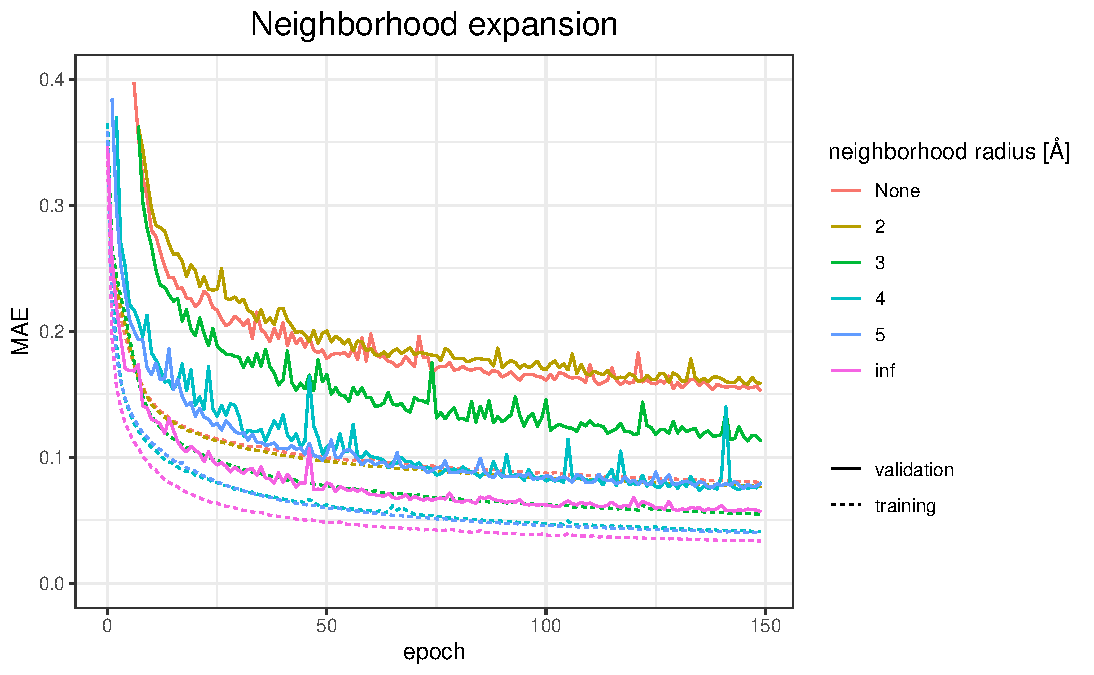
\includegraphics[width=\linewidth]{figures/neighborhood-expansion}
	
	\caption{The learning curves with different neighborhood radii are show over the courses of 150 epochs. The color corresponds to the neighborhood radius. Dotted lines show the training- and solid lines the validation errors. Note that for each radius, there is a training- and a validation-error curve. Each curve is an average of three learning curves with the same neighborhood radius. All curves were generated using a simple optimization scheme described in Section~\ref{sec:training}. Both, validation- and training-error could be lowered considerably by employing a more sophisticated optimization scheme. However, this would be at the expense of comparability between curves (see Section~\ref{sec:training}).}
	\label{fig:neighborhood-expansion}
\end{figure}

As Figure~\ref{fig:neighborhood-expansion} shows, the best performance is indeed achieved with the complete graph - connecting every atom with every other atom in the molecule with an edge. In general, the larger the neighborhood radius, the better the performance. This result is in line with the suspicion that the real reason for the good performance of Tencent Lab's model is the addition of new edges rather than the addition of the euclidean distance feature.
The result is somewhat counterintuitive and in contrast with the principle of graph-convolution. As described in the introduction, in theory, graph convolutions update node-representation based on the local neighborhood of each node. Eventually, after $t$ layers, each node representation would contain indirect contributions from all other nodes with $t$ or fewer edges apart. However, the results at hand show that the performance is best if the graph convolution considers all atoms at every layer. This contrast between theory and empiric results clearly shows that much remains to be discovered about the use of GCNNs for molecules.

For small molecules and with considerable computational power available, one could simply accept this finding as it is and represent molecules as complete graphs. However, for larger molecules with hundreds of atoms, this would be computationally not feasible as the number of edges increases quadratically ($\frac{n(n - 1)}{2}$ edges for $n$ nodes). Therefore, the next experiments will aim at finding an alternative way that captures the advantage of the complete graph-approach without the excessively high computational cost.

%Cite Alchemy paper and point out that the high-performing kaggle-teams all use fully connected graphs.
%Does no one notice?


\subsection{Introducing a graph-state as added input in every message-passing step does not improve results}
\label{sec:root-node}


What the usage of complete graphs in graph convolutional networks essentially does is to ensures that during every node update, a representation of every other node in the graph contributes to the update - even nodes that are too far away to have any direct interaction with the updated node (atom).
A possible explanation of this behavior is that the node update benefits from having access to information about the whole graph (molecule). This interpretation begs the question if a similar effect can be achieved by a different architecture (that does not require the use of computationally prohibitive complete graphs).

An interesting experiment to test this hypothesis is to include graph-level information at every node update (without having to use complete graphs.) One such idea is the use of a root node. A root node (called master node in Gilmer et. al.~\cite{Gilmer2017}) is a virtual node that is connected to every other node in the graph. In the molecule case, the root node does not represent a real atom. Instead, it can be used to represent information about the whole molecule. Then, as every node is connected to the root node, every node update has access to information about the whole molecule. On could initialize the root node representation with molecule level features (such as number of atoms, electric dipole, etc.). However, all those features are implicit in the 3D molecular structure. Sticking to the pure deep learning philosophy, the root node representation can also be learned solely from the raw data.

Ideally, the use of such a root node would allow to achieve a similar performance as when using complete graphs without the high computational cost - while the number of edges increases quadratically with the number of nodes in the complete graph, the root node only introduces one new edge per node. At the very least, the negative effect of decreasing performance with decreasing neighborhood radius shown in Figure~\ref{fig:neighborhood-expansion} should be less pronounced if the root node has the desired effect.

\begin{figure}[H]
	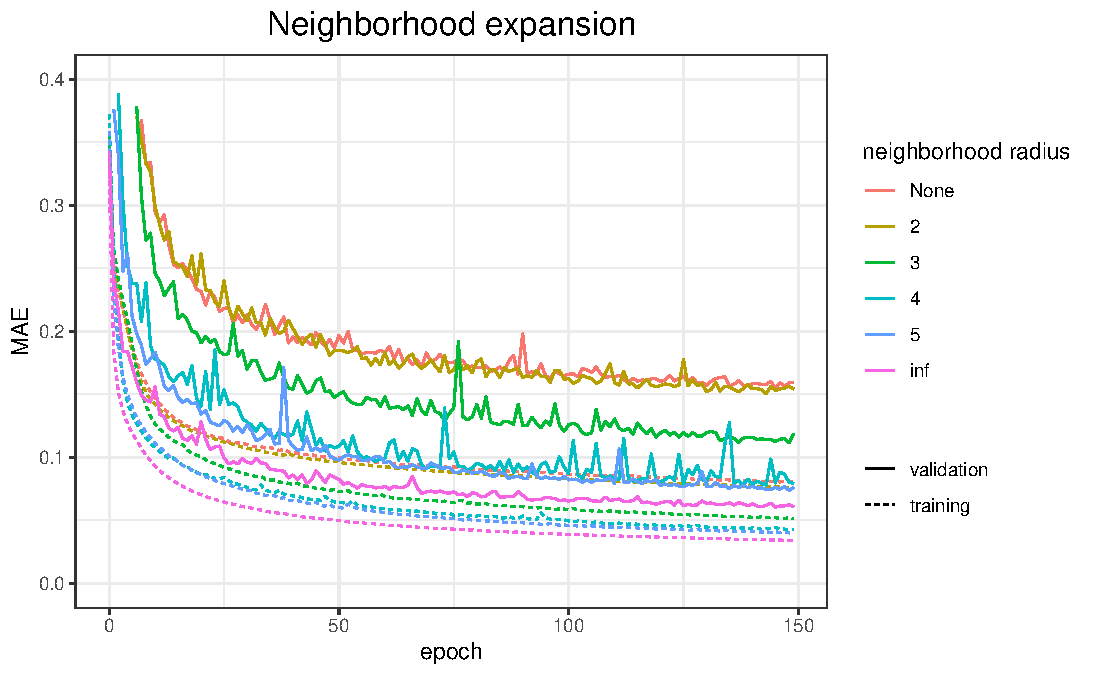
\includegraphics[width=\linewidth]{figures/neighborhood-expansion-root-weight}
	\caption{The results illustrated by this figure have been produced in exactly the same manner as Figure~\ref{fig:neighborhood-expansion} with the addition of a root node as the only difference. This allows a direct comparison between the figures such that any difference could be attributed to the presence or absence of a root node. The results show no difference beyond stochastic variation thus indicating that the addition of a root node is no substitute to the use of complete graphs when representing molecules.}
	\label{fig:neighborhood-expansion-root-weight}
\end{figure}

Figure~\ref{fig:neighborhood-expansion-root-weight} show the same experiment as Figure~\ref{fig:neighborhood-expansion} with the addition of a root node as the only difference (Section~\ref{sec:mpnn-architecture} describes how the concept of the root node is implemented in practice in the model at hand). Unfortunately, there is no noticeable difference between the results of the two experiments. This indicates that the superior performance of complete graphs is not solely due to the fact that every node update includes input from the whole molecule. A possible reason for the failure of the root node to replace a complete graph approach could be that the root node cannot contribute geometric information about non-neighboring atoms. On the other hand, in the complete graph, each node's representation is considered in the update only in conjunction with the it's distance from the updated node. Recall Equation~\ref{eq:message-function} which defines the message from a node to another node as a function of both nodes as well as the connecting edge. While a root node representation can encode information about the whole molecule, such as number and types of atoms, their position relative to the updated node (atom) is missing.


\subsection{Excluding hydrogen atoms from the molecule-graph speeds up training but increases the error}
\label{sec:no-hydrogens}

Another possible preprocessing step is to disregard hydrogen atoms and instead add the number of hydrogen atoms bonded to a given heavy atom as a node feature. The rational behind this step is that the chemical properties of hydrogen atoms depend strongly on the heavy atom to which it is bound. While some information is lost during this step, the average number of atoms in the molecule is reduced by an average factor of
%21.61315346375882 ->
%9.712215362411802
%
%455.46524214239895 ->
%84.99518922386144
from 21.6 to 9.7 in the training-set. This modest reduction in the number of nodes leads to a very dramatic reduction in the number of edges. Naturally, this effect is most pronounced in complete graphs where the number of edges increases quadratically with the number of nodes ($\frac{n(n - 1)}{2}$ edges for $n$ nodes). While the average number of edges using complete graphs is 455.5 in the training-set, this number drops to 85 after excluding hydrogen atoms. Thus the data representation becomes much more compact leading to a dramatic decrease in training time from around three minutes per epoch to only 0.9 minutes. This is a strong incentive to investigate whether ignoring hydrogen atoms in the molecular structure is a viable option. Figure~\ref{fig:implicit-hydrogens} clearly shows that this is not the case. The loss is far higher when using the hydrogen-less structure compared to the full structure. Similar findings have also been reported in the literature~\cite{Gilmer2017}. For these reasons, every other experiment in this thesis uses full structures including hydrogen atoms.

\begin{figure}[H]
	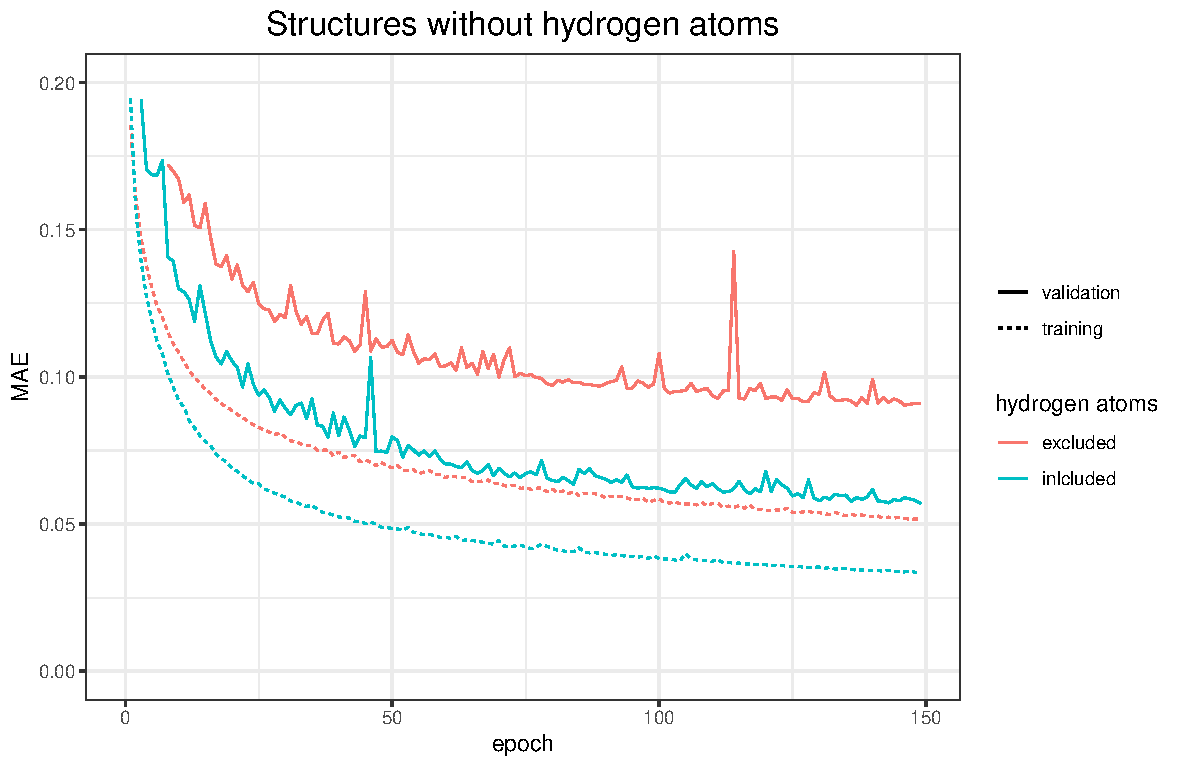
\includegraphics[width=\linewidth]{figures/implict-hydrogens.pdf}
	\caption{Input graphs with (explicit representation) and without hydrogen atoms(implicit representation). The model architecture is exactly the same for both learning curves such that the lacking hydrogen atoms are the only factor causing the considerable difference. The result show clearly the importance of including hydrogen atoms in the graph representation of organic molecules.}
	\label{fig:implicit-hydrogens}
\end{figure}

\paragraph{Further information: Why a hydrogen-less structure contains implicit information about hydrogen atoms}
Despite dropping all hydrogen atoms from the molecule structure, the information how many hydrogen atoms there are and to which atoms they are bound is still implicitly contained in the structure. (For the same reason, hydrogen atoms are also excluded from standard molecule graphs as the one shown in Figure~\ref{fig:caffeine}.) In short, it is a way of summarizing raw data which speeds up training considerably while loosing some information. The reason it can be called 'implicit hydrogen representation' is that the information how many hydrogens (but not their exact position) is inherent in the structural information given all the other atoms and the bonds between them. The only piece of knowledge from organic chemistry required to understand this is that every given atom type, such as carbon or oxygen, only engages in a fixed number of bonds: four for carbon, two for oxygen, one for hydrogen, etc. (with double or triple bonds counting twice or trice, respectively). This number is called valence and is dependent on the number of electrons in the outer orbital - called valence electrons~\cite{Organic-chemistry}. In a molecular structure without hydrogen atoms, the number of bonds to heavy atoms (i.e. non-hydrogen atoms) is given for each atom as the number of it's neighbor nodes. The number of hydrogen atoms bound to any given atom is thus it's valence minus the number of neighbor nodes. It is for this reason that omitting hydrogens from the structure can be thought of as equivalent to adding the feature 'number of hydrogen atoms' to each heavy atom. Note that while this number is implicit in the structure, the exact position of the hydrogen atoms is lost when they are omitted from the structure.



\subsection{Graph-convolution layers with independent weights give the same results as with shared weights}
\label{sec:weight-sharing}

Recall the message function $M_t$ and the (node-)update-function $U_t$ defined in Equation~\ref{eq:message-function} and~\ref{eq:update-function}, respectively. In this general definition, each graph-convolution layer (each message passing step) $t$ has it's own $M_t$ and $U_t$. However, in most implementations of GCNNs, $M_t = M~~\forall~t$ and $U_t = U~~\forall~t$ which simplifies the two equations~\ref{eq:message-function} and~\ref{eq:update-function} to

\begin{equation}
m_v^{t+1} = \sum_{w \in N(v)} M(h_v^t, h_w^t, e_{vw})
\end{equation}
\label{eq:message-function-shared}

and

\begin{equation}
h_v^{t+1} = U(h_v^t, m_v^{t+1}).
\end{equation}
\label{eq:update-function-shared}

% TODO: cite

In plain English, this means that the weights between the graph-convolution layers (message passing steps) are shared. This allows for efficient training and works well in practice. However, there is no theoretical reason that weight sharing is necessarily superior. For instance, it would be conceivable that independent weights would work better for extracting different kinds of features at different graph-convolution layers. Recall that in the first graph-convolution layer, the input for a given node update consists only of direct neighbor nodes, at the second layer, the update indirectly contains information from all second-degree neighbor nodes, etc. Hence, learning different weights for different graph-conv layers might be beneficial. Note also that in regular convolutional networks used for computer vision, every layer has independent weights even within blocks of convolutional layers with the same dimension (where weight sharing would be possible in theory). It is therefore far from clear that weight sharing has to be the preferred approach for graph-convolution.

In order to investigate the possible benefit of independent weights, the next experiment compares the MPNN described in~Section\ref{sec:base-architecture} with an architecture without weight sharing. The two architectures are identical in every other aspect to allow isolate the effect of weight sharing. Figure~\ref{fig:weight-sharing} shows that there is no noticeable difference between the learning curves.


\begin{figure}[H]
	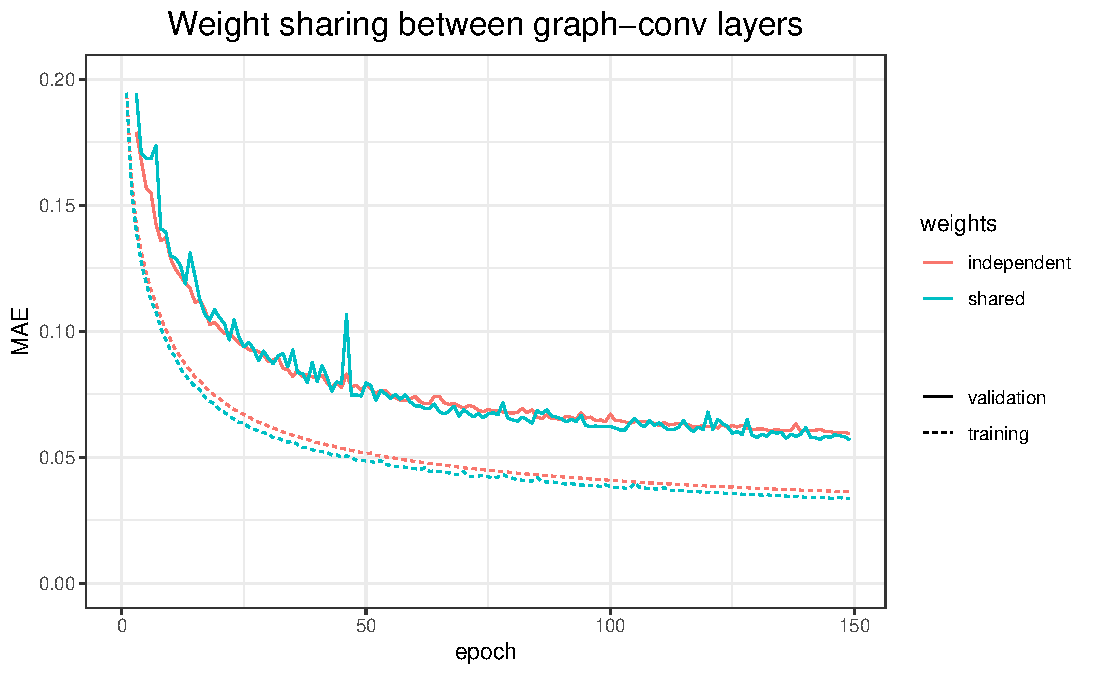
\includegraphics[width=\linewidth]{figures/weight-sharing.pdf}
	\caption{The result of using independent weights between graph-conv layers is the same as when using weight-shared layers. Note that the two architectures are identical in every other way apart from weight-sharing of graph-conv layers. Complete graphs were used as the input data as this was shown to be the best performing transformation in earlier experiments (Section~\ref{sec:neighborhood-expansion}). All curves were generated using a simple optimization scheme described in Section~\ref{sec:training}.}
	\label{fig:weight-sharing}
\end{figure}


Another interesting observation is that the learning curves are identical not only in terms of the lowest MAE they achieve but also in the speed at which the converge on this MAE. It would not have been surprising for the independent weights to require more training time as each graph-convolution layer's weights are only updated once for a given batch in a given epoch. In weight-sharing architectures on the other hand, the graph convolution-layer is updated $n$ times for each batch and epoch in a model with $n$ convolution-layers. Nevertheless, Figure~\ref{fig:weight-sharing} clearly shows that the two approaches are equal in terms of training-time.

One caveat worth mentioning is that only because independent weights were not found to be beneficial for the architecture at hand does this not mean that they will never be beneficial in other architectures.

Furthermore, while we can see that they do not decrease the loss, we still do not know why exactly that is the case. This question is not addressed frequently in the literature - rather the use of weight-sharing is most commonly accepted without much investigation into why it's used. In contrast, we would not even think about sharing weights across regular convolution-layers for a computer vision task. It is far from obvious why there is no difference between shared and independent weights in GCNNs. Finding out why this is the case might also lead to insights about how to build better GCNN architectures.  

Summing up, the results confirm the common practice of using weight-sharing across graph-convolution layers but the question why weight-sharing works in GCNNs is still left open and worth investigating.


\subsection{Manual feature engineering does not improve results compared to using only raw input data}
\label{sec:raw-data}

The previous experiments included some hand-crafted features calculated with the computation chemistry python library \textit{rdkit}~\footnote{\url{https://www.rdkit.org}}. This was done in order replicate the approach of Chen et. at.~\cite{Chen2019} In the literature, there are conflicting indications about the uses of manually engineered chemical features as input for MPNNs. For instance, the three best solutions of the \textit{Alchemy} competition show almost equally good results~\footnote{\url{https://alchemy.tencent.com}} but differ in their assessment of the benefit of manually calculated chemical features. While the winning model uses such features and the authors claim that they improved their results, the second and third solutions (with virtually the same performance) state that adding manually engineered features gave no benefit and were thus not used~\cite{Klicpera2019}~\footnote{
\textit{Alchemy} competition winners: \\
	1\textsuperscript{th}: \url{https://alchemy.tencent.com/data/2019/1st_solution-ape-MPNN_NJU_Chem.pdf} \\
	2\textsuperscript{nd}: \url{https://alchemy.tencent.com/data/2019/2nd_solution-SchNet_and_SchNet_with_Edge_Updates_1117.pdf}\\
	3\textsuperscript{rd}: \cite{Klicpera2019}
}.
In most cases, the literature lacks a direct comparison between using only raw data (atom-type, position and edges) and adding manually computed features. It is therefore often hard to deduce whether the good results are due to an effective model architecture or due to the smartly engineered chemical features used as input.

The next experiment trains two almost identical GCNNs: one uses the same chemical features as Chen et. at.~\cite{Chen2019} while the other one uses only atom-type, edge-type and distance as input. The two nets are identical in every aspect except of course for the different dimension of the input layer. All chemical features~\footnote{
	The chemical atom (node) feature are comprised of three boolean variables indicating whether the atom is an electron donor, an electron acceptor and whether it is part of an aromatic ring. Furthermore, they include a categorical variable indicating the hybridization type. As all of those are simply functions of the atom-type or the local structure, it comes as no surprise that they are redundant.
	
}
are computed from the structure without additional information. Hence - if they are relevant for predicting the target variable - they are exactly the kind of information that the graph-convolution layers should extract from the structure. If that's the case, the addition of the computed chemical features is expected to have no effect on the model's loss. Indeed, Figure~\ref{fig:raw-data} shows no difference between the two models.

\begin{figure}[H]
	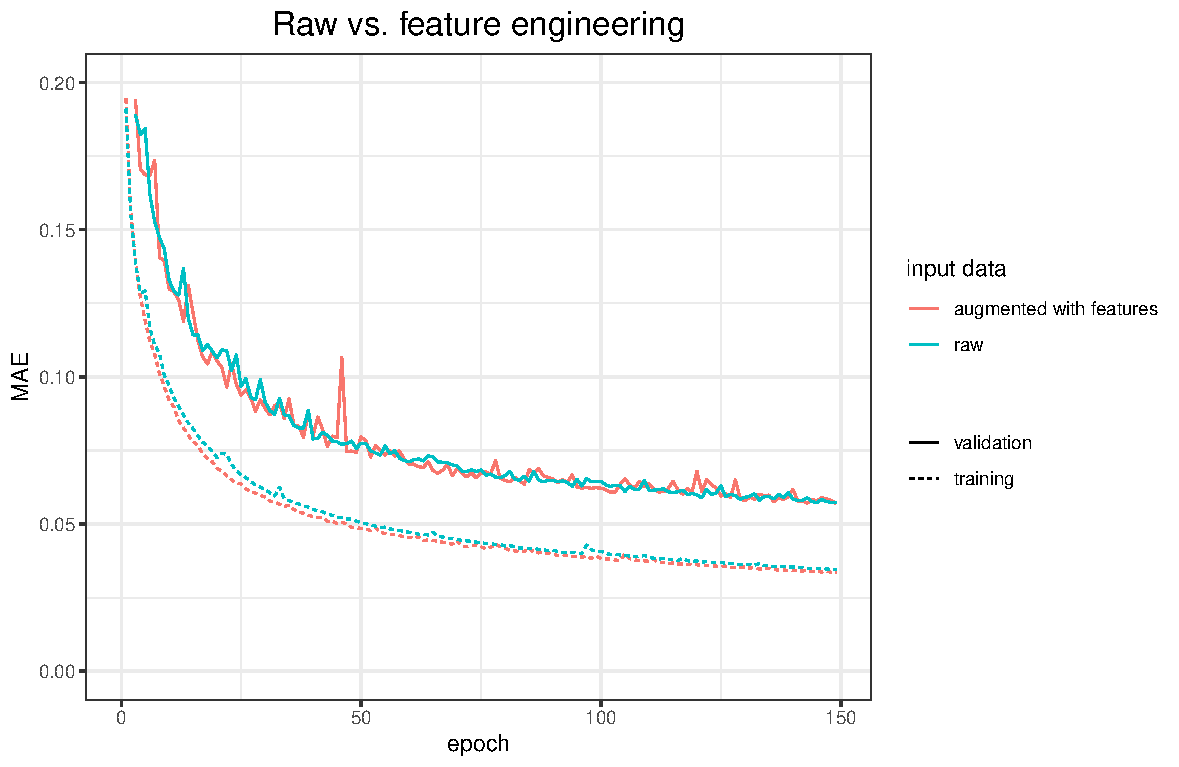
\includegraphics[width=\linewidth]{figures/raw-data}
	\caption{Raw data alone gives as good results as with manually engineered features. As in the previous experiments, each line is an average of three independent learning curves using the simple optimization scheme described in Section~\ref{sec:training}.}
	\label{fig:raw-data}
\end{figure}

Therefore, we can conclude that the graph-convolution layers are able to extract relevant chemical information to predict the target variable. The results do not preclude that another architecture might benefit from the addition of computed chemical features or that more and more sophisticated manually engineered features might even provide some benefit for the model at hand. Nevertheless, the results show that manual feature engineering is far from essential and strengthen the believe that the deep-learning approach of using raw data instead of manual feature engineering is also preferable for chemical applications of GCNNS.

All further experiments are conducted without calculated chemical features and only use the raw structural data instead.


\subsection{Direction vectors as edge features have no impact}
\label{sec:direction-vectors}

It stands to reason that one of the main limitations of using graph neural networks for data embedded in spacial dimensions is the loss of a part of spacial information as explained in Section~\ref{sec:lack-of-3d-structure}. (While this thesis focuses on molecules, representing any other three-dimensional data as graphs would be suffer from the same limitation).
	
In an attempt to address this limitation, an additional (vector-valued) edge-feature was included as input into the message-function $M_t$ (Equation~\ref{eq:message-function}): the direction vector from the sending atom $h_v$ to the receiving (i.e. to be updated) atom $h_w$ was added to the features of edge $e_{vw}$. This vector is invariant to translation of the molecule making it potentially more informative than using raw atom-coordinates as raw features~\footnote{Adding the raw coordinate values to the node features gave no improvement at all. As this is expected given that the coordinates depend on the arbitrary positioning and rotation of the coordinate system, the results are not shown here.} However, the direction vector is still not invariant to the arbitrarily chosen rotation of molecule in the coordinate system.

In order to provide the direction vector with some useful information, the molecule's center was chosen as the origin of coordinate system. Thanks to this transformation, a direction vector $pos(h_w) - pos(h_v)$ from atom $h_v$ to atom $h_w$ always provides the information if $h_v$ lies closer to the center (positive values) or closer to the periphery of the molecule (negative values) in relation to $h_w$.

\begin{figure}[H]
	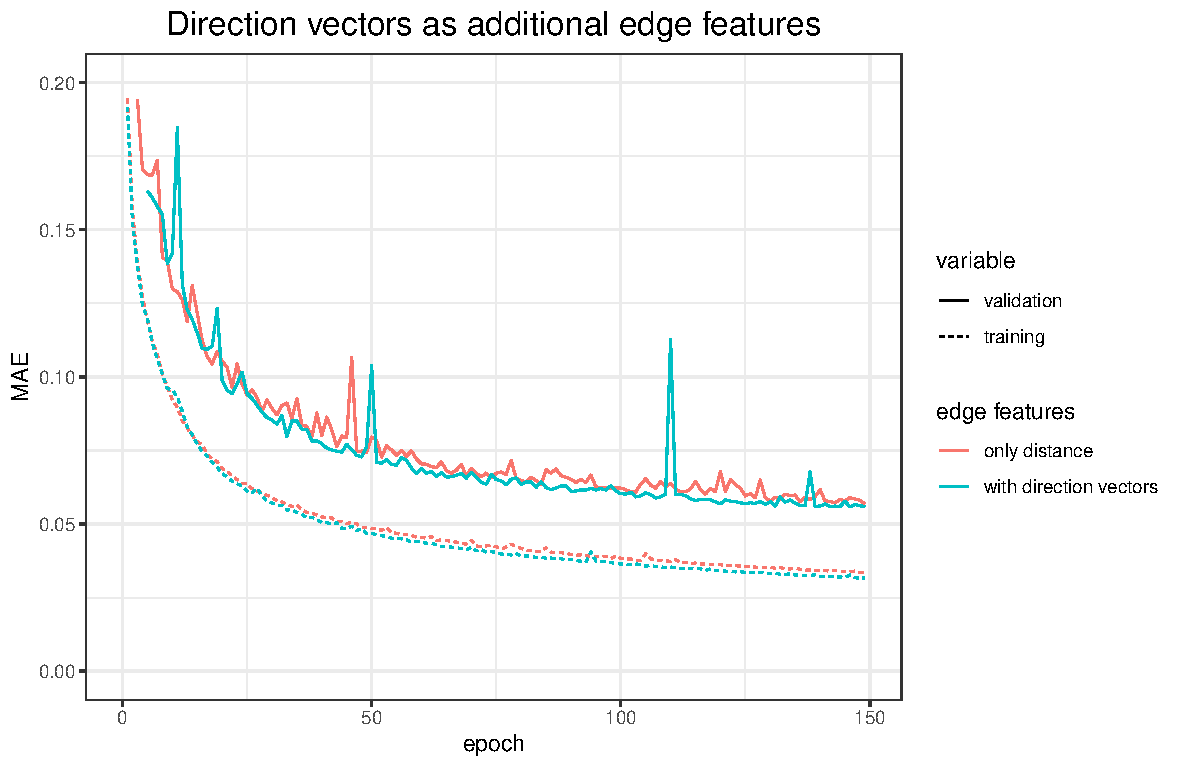
\includegraphics[width=\linewidth]{figures/edge-direction-vectors}
	\caption{Direction vectors as edge features do note improve the results. As in the previous experiments, each line is an average of three independent learning curves and were obtained using the simple optimization scheme described in Section~\ref{sec:training}.}
	\label{fig:edge-direction-vectors}
\end{figure}

For this reason, the direction vector could contain useful information despite the lack of rotational invariance. Nevertheless, no improvement was achieved by the addition of the direction vector to the edge features as shown in Figure~\ref{fig:edge-direction-vectors}. The results do not give evidence whether the additional edge features do not contain relevant information at all or whether the graph-convolution was just not able to extract useful higher-level features from this information. The possibility that another graph-convolution architecture might benefit from using direction vectors as edge-features cannot be ruled out completely but the results at hand do not provide evidence for it.

An interesting attempt at modeling 3D structural information in GCNNs is made in the 3D-embedded graph convolutional network of Cho et. al.~\cite{Cho2018}. However, upon closer inspection the approach seems to suffer from same issue as the experiment above that the input data is not invariant to the arbitrary rotation of the molecule. Adapting this model to and applying it to the \textit{Alchemy} dataset gave only disappointing results. After 200 epochs, the validation MAE plateaued at around 1.8 which is about three times higher than the validation MAE achieved with the models based on Tencent's simple MPNN~\cite{Chen2019} used for the other experiments in this thesis. Even the training error did not even go below the validation error achieved with the simple MPNN but plateaued at around 0.85.






